\documentclass[xetex,mathserif,serif,aspectratio=169]{beamer}

\usepackage{xltxtra}
\usepackage{color}
\usepackage{url}
\usepackage{listings}
\usepackage{fontspec}
\usepackage{geometry}
\usepackage{lastpage}
\usepackage{fancyhdr}
\usepackage{amsmath}
\usepackage{amsthm}
\usepackage{amssymb}
\usepackage{blkarray}
\usepackage{multicol}
\usepackage{relsize}
\usepackage{listings}
\usepackage{xunicode}
\usepackage{xltxtra}
\usepackage{color}
\usepackage{url}
\usefonttheme[onlymath]{serif}

\definecolor{solarized@base03}{HTML}{002B36}
\definecolor{solarized@base02}{HTML}{073642}
\definecolor{solarized@base01}{HTML}{586e75}
\definecolor{solarized@base00}{HTML}{657b83}
\definecolor{solarized@base0}{HTML}{839496}
\definecolor{solarized@base1}{HTML}{93a1a1}
\definecolor{solarized@base2}{HTML}{EEE8D5}
\definecolor{solarized@base3}{HTML}{FDF6E3}
\definecolor{solarized@yellow}{HTML}{B58900}
\definecolor{solarized@orange}{HTML}{CB4B16}
\definecolor{solarized@red}{HTML}{DC322F}
\definecolor{solarized@magenta}{HTML}{D33682}
\definecolor{solarized@violet}{HTML}{6C71C4}
\definecolor{solarized@blue}{HTML}{268BD2}
\definecolor{solarized@cyan}{HTML}{2AA198}
\definecolor{solarized@green}{HTML}{859900}
\definecolor{yaleblue}{HTML}{0E4C92}

\newcommand{\yellow}[1]{\textcolor{solarized@yellow}{#1}}
\newcommand{\orange}[1]{\textcolor{solarized@orange}{#1}}
\newcommand{\red}[1]{\textcolor{solarized@red}{#1}}
\newcommand{\magenta}[1]{\textcolor{solarized@magenta}{#1}}
\newcommand{\violet}[1]{\textcolor{solarized@violet}{#1}}
\newcommand{\blue}[1]{\textcolor{solarized@blue}{#1}}
\newcommand{\cyan}[1]{\textcolor{solarized@cyan}{#1}}
\newcommand{\green}[1]{\textcolor{solarized@green}{#1}}
\newcommand{\yblue}[1]{\textcolor{yaleblue}{#1}}
\newcommand{\base}[1]{\textcolor{solarized@base01}{#1}}


\defaultfontfeatures{Mapping=tex-text}
\hypersetup{pdfstartview={FitH}}

\newcommand{\old}[1]{\fontspec[Alternate=1,Ligatures={Common}]{Hoefler Text}\fontsize{18pt}{30pt}\selectfont #1}%
\newcommand{\oldA}[1]{\fontspec[Alternate=1,Ligatures={Common, Rare}]{Hoefler Text}\fontsize{12pt}{15pt}\selectfont #1}%
\newcommand{\oldB}[1]{\fontspec[Ligatures={Common}]{Didot}\fontsize{12pt}{15pt}\color{solarized@base02}\selectfont #1}%
\newcommand{\tfont}[1]{\fontspec[Alternate=1,Ligatures={Common}]{Hoefler Text}\fontsize{12pt}{20pt}\selectfont #1}%
\newcommand{\dfont}[1]{\fontspec[Ligatures={Common}]{Didot}\fontsize{12pt}{12pt}\selectfont #1}%

\setbeamerfont{title}{family=\old}
\setbeamerfont{author}{family=\tfont}%
\setbeamerfont{frametitle}{family=\oldA}
\setbeamerfont{date}{family=\dfont}

\setbeamertemplate{navigation symbols}{}
\setbeamertemplate{footline}[text line]{%
  \parbox{0.99\linewidth}{
    \normalsize\vspace*{-24pt}\hfill{\color{solarized@base00}\insertframenumber/\inserttotalframenumber}
  }
}


\setlength{\parindent}{0pt}
\setlength{\parskip}{12pt}

\setbeamercolor{structure}{bg=solarized@base3, fg=solarized@base02}
\setbeamercolor{titlelike}{fg=solarized@cyan}
\setbeamercolor{title}{fg=solarized@blue}
\setbeamercolor{subtitle}{fg=solarized@magenta}
\setbeamercolor{alerted text}{fg=orange}
\setbeamercolor{itemize}{fg=solarized@base02}
\setbeamercolor{background canvas}{bg=solarized@base3}
\setbeamercolor{enumerate subitem}{fg=solarized@base02}

\newcommand{\minimize}{\mathop{\mathrm{minimize}}}
\newcommand{\argmin}{\mathop{\mathrm{arg\,min}}}
\newcommand{\argmax}{\mathop{\mathrm{arg\,max}}}
\newcommand{\st}{\mathop{\mathrm{subject\,\,to}}}


\usepackage[]{algorithm2e}
\usepackage{../kbordermatrix}

\begin{document}

%%%%%%%%%%%%%%%%%%%%%%%%%%%%%%%%%%%%%%%%%%%%%%%%%%%
\begin{frame}[fragile] \frametitle{} \oldB \small

\vfill

{\fontsize{0.7cm}{0cm}\selectfont Lecture 15 \\\vspace{0.2cm} Weight Initialization,
Momentum and Learning Rates}\\\vspace{0.5cm}
09 March 2016

\vspace{2cm}

\begin{minipage}{0.6\textwidth}
Taylor B. Arnold \\
Yale Statistics \\
STAT 365/665
\end{minipage}
\hfill
\begin{minipage}{0.3\textwidth}\raggedleft

\includegraphics[scale=0.3]{../yale-logo.png}
\end{minipage}%

\end{frame}

%%%%%%%%%%%%%%%%%%%%%%%%%%%%%%%%%%%%%%%%%%%%%%%%%%%
\begin{frame}[fragile] \frametitle{} \oldB \small

Notes:
\begin{itemize}
\item Problem set 5 is due on Monday, March 14th
\end{itemize}

\end{frame}

%%%%%%%%%%%%%%%%%%%%%%%%%%%%%%%%%%%%%%%%%%%%%%%%%%%
\begin{frame}[fragile] \frametitle{} \oldB \small

\begin{itemize}
\item Today:
\begin{itemize}
\item modular neural networks
\item a bit of review
\item initializing weights
\item quasi second order SGD
\item learning rate schedule
\item hyper-parameter selection heuristics
\end{itemize}
\end{itemize}

\end{frame}

%%%%%%%%%%%%%%%%%%%%%%%%%%%%%%%%%%%%%%%%%%%%%%%%%%%
\begin{frame}[fragile] \frametitle{} \oldB \small

\textbf{\yblue{Modular view of neural networks}}

We have so far thought of neural networks as being primarily
defined by a network of individual neurons. This is helpful
both for its simplicity and the historical development of the
estimators. However, there is another way of thinking about
neural networks that more closely mimics popular implementations
such as Caffe, Keras, and Torch.

\end{frame}

%%%%%%%%%%%%%%%%%%%%%%%%%%%%%%%%%%%%%%%%%%%%%%%%%%%
\begin{frame}[fragile] \frametitle{} \oldB \small

\textbf{\yblue{Modular view of neural networks, cont.}}

For an input vector $x$ and a response $y$, we can view the network
as simply being something like:
\begin{align}
z^1 &= W^1 a^0 + b^1 \\
a^1 &= \sigma(z^1) \\
z^2 &= W^2 a^1 + b^2 \\
a^2 &= \sigma(z^2) \\
z^3 &= W^3 a^2 + b^3 \\
a^3 &= \sigma(z^3) \\
\text{Cost} &= (y - a^3)^2
\end{align}
\pause Each level can be described by a \textit{module}. The $z$ layers
are called linear layers, the $a$'s as sigmoid layers, and the last
line is simply the cost function. Notice that the activation functions
are now their own layers, which actually simplifies things mathematically.

\end{frame}

%%%%%%%%%%%%%%%%%%%%%%%%%%%%%%%%%%%%%%%%%%%%%%%%%%%
\begin{frame}[fragile] \frametitle{} \oldB \small

\textbf{\yblue{Modular view of neural networks, cont.}}

Each type of module needs to be able to:
\begin{itemize}
\item take an input and return an output for the current tuning parameters
\item calculate the matrix $\frac{\partial \text{output}_i}{\partial \text{input}_j}$
\item calculate the set $\frac{\partial \text{output}_i}{\partial \text{parameters}_j}$
\item store the tuning parameters
\item update parameters from a minibatch
\end{itemize}
If I have all of these implemented, I can simply chain together
modules and have a built-in algorithm for learning from input data.

\end{frame}

%%%%%%%%%%%%%%%%%%%%%%%%%%%%%%%%%%%%%%%%%%%%%%%%%%%
\begin{frame}[fragile] \frametitle{} \oldB \small

\textbf{\yblue{Modular view of neural networks, cont.}}

An example, using the \textbf{keras} library, describes this
well:
\begin{verbatim}
model = Sequential()
model.add(Dense(64, input_dim=20, init='uniform'))
model.add(Activation('sigmoid'))
model.add(Dropout(0.5))
model.add(Dense(64, init='uniform'))
model.add(Activation('sigmoid'))
model.add(Dropout(0.5))
model.add(Dense(10, init='uniform'))
model.add(Activation('softmax'))
\end{verbatim}
Where dense refers to a linear connected layer.

\end{frame}


%%%%%%%%%%%%%%%%%%%%%%%%%%%%%%%%%%%%%%%%%%%%%%%%%%%
\begin{frame}[fragile] \frametitle{} \oldB \small

\textbf{BVLC GoogLeNet:} Szegedy et al. (2014)

\begin{center}
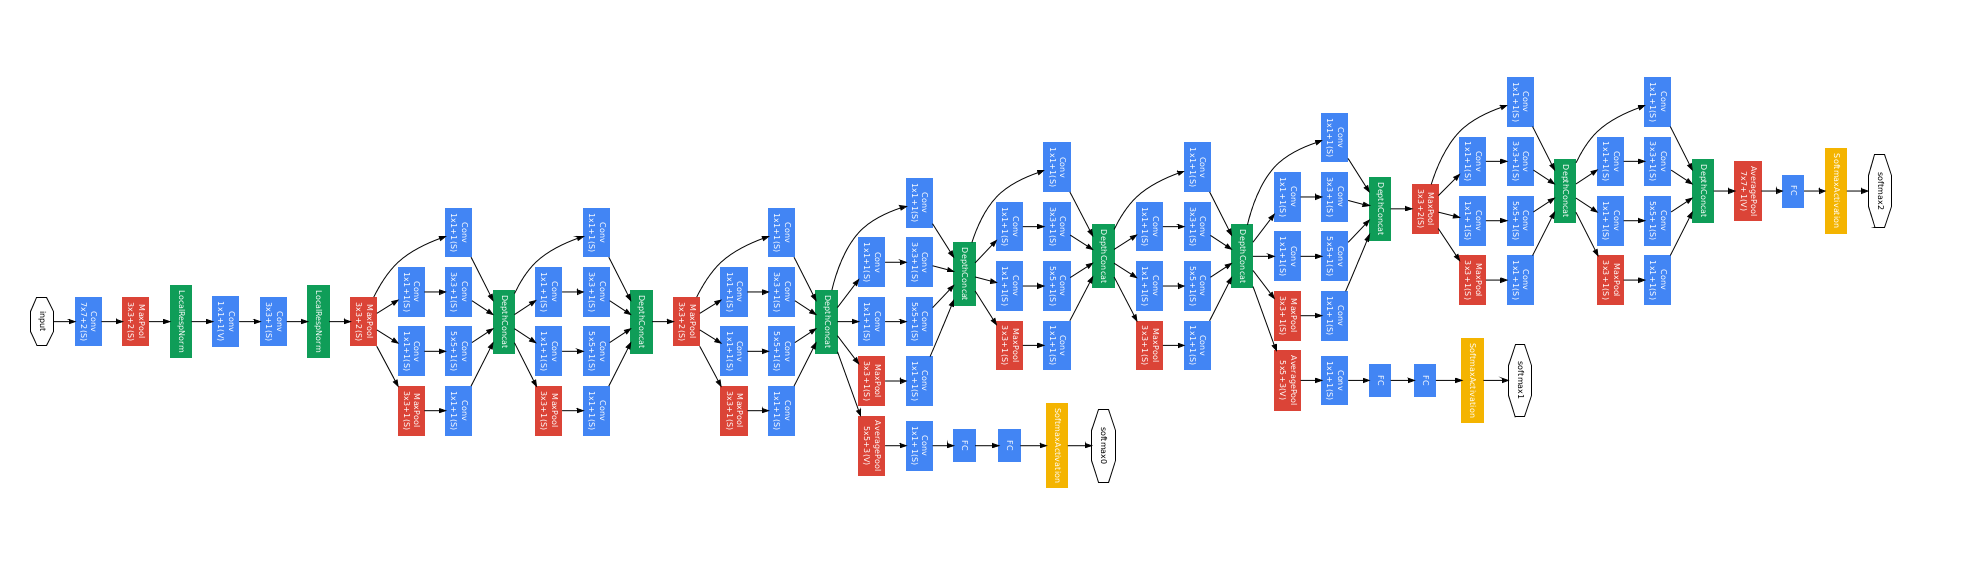
\includegraphics[width=\textwidth]{img/googlenet_diagram.png}
\end{center}

\end{frame}

%%%%%%%%%%%%%%%%%%%%%%%%%%%%%%%%%%%%%%%%%%%%%%%%%%%
\begin{frame}[fragile] \frametitle{} \oldB \small

\textbf{\yblue{Review: Cross-entropy and soft-max}}

Due to the shape of the sigmoid neuron, weights that are very far from
their optimal values learn slowly in a plain, vanilla network. One way
to fix this is to use the cross-entropy cost-function, defined as:
\begin{align*}
C &= - \sum_j \left[ y_j \log(a_j^L) + (1-y_j) \log(1 - a_j^L) \right]
\end{align*}
For a single sample, and similarly for an entire mini-batch.

Another common approach is to define what is termed a softmax layer.
The redefines the activations of the output later, $a^L$, as follows:
\begin{align*}
a^L_j &= \frac{e^{z_j^L}}{\sum_k e^{z_k^L}}
\end{align*}
This has the additional benefit that the last layer is easily interpreted
as a sequence of probabilities.

\end{frame}

%%%%%%%%%%%%%%%%%%%%%%%%%%%%%%%%%%%%%%%%%%%%%%%%%%%
\begin{frame}[fragile] \frametitle{} \oldB \small

\textbf{\yblue{Review: Regularization in Neural Networks}}

As the size of neural networks grow, the number of weights and biases can
quickly become quite large. State of the art neural networks today often
have billions of weight values. In order to avoid over-fitting, one common
approach is to add a penalty term to the cost function. Common choices are
the $\ell_2$-norm, given as:
\begin{align*}
C &= C_0 + \lambda \sum_i w_i^2
\end{align*}
Where $C_0$ is the unregularized cost, and the$\ell_1$-norm:
\begin{align*}
C &= C_0 + \lambda \sum_i |w_i|.
\end{align*}
The distinction between these is similar to the differences between lasso and
ridge regression.

\end{frame}

%%%%%%%%%%%%%%%%%%%%%%%%%%%%%%%%%%%%%%%%%%%%%%%%%%%
\begin{frame}[fragile] \frametitle{} \oldB \small

\textbf{\yblue{Review: Dropout}}

A very different approach to avoiding over-fitting is to use an approach called
\textit{dropout}. Here, the output of a randomly chosen subset of the neurons
are temporarily set to zero during the training of a given mini-batch. This makes
it so that the neurons cannot overly adapt to the output from prior layers as
these are not always present. It has enjoyed wide-spread adoption and massive
empirical evidence as to its usefulness.

\end{frame}

%%%%%%%%%%%%%%%%%%%%%%%%%%%%%%%%%%%%%%%%%%%%%%%%%%%
\begin{frame}[fragile] \frametitle{} \oldB \small

\textbf{\yblue{Initial weights}}

Rather than initializing the weights in the neural network by a standard normal
Gaussian, it is better to initialize with Gaussian noise with zero mean but a
standard deviation of $1 / \sqrt{n}$ where $n$ is the number of nodes from the
previous layer that are incoming to this given node. This perhaps makes sense
when we consider two layers of a neural network:

\begin{align}
z^1 &= W^1 a^0 + b^1 \\
a^1 &= \sigma(z^1)
\end{align}

This has the effect of making the distribution of all of the weighted inputs, $z_j^l$,
equal to standard Gaussian noise.

\end{frame}

%%%%%%%%%%%%%%%%%%%%%%%%%%%%%%%%%%%%%%%%%%%%%%%%%%%
\begin{frame}[fragile] \frametitle{} \oldB \small

\textbf{\yblue{Optimization tricks}}

For the rest of today, I am going to talk about approaches for fitting neural
networks that can apply more generally to difficult optimization problems.
I think it is easier to use a simple example to illustrate this, rather than
directly applying to neural networks. So we'll return to minimizing the sum
of squared residuals in a linear models:
\begin{align*}
f(\beta) &= \frac{1}{n} \sum_i (y_i - x_i^t \beta)^2 \\
&= \frac{1}{n} \left( y^t y + \beta^t X^tX \beta - 2 y^t X \beta \right)
\end{align*}
With the analytic gradient of:
\begin{align*}
\nabla f(\beta) &= 2 X^t X \beta - 2 y^t X
\end{align*}

\end{frame}

%%%%%%%%%%%%%%%%%%%%%%%%%%%%%%%%%%%%%%%%%%%%%%%%%%%
\begin{frame}[fragile] \frametitle{} \oldB \small

\textbf{\yblue{Gradient Descent}}

Gradient Descent uses the following set of updates for
some learning rate $\eta > 0$:
\begin{align*}
\beta_{t+1} &= \beta_{t} - \eta \cdot \nabla f(\beta_t)
\end{align*}
Which can be re-written into two parts:
\begin{align*}
v_{t+1} &= - \eta \cdot \nabla f(\beta) \\
\beta_{t+1} &= \beta_{t} + v_{t+1}.
\end{align*}

\end{frame}


%%%%%%%%%%%%%%%%%%%%%%%%%%%%%%%%%%%%%%%%%%%%%%%%%%%
\begin{frame}[fragile] \frametitle{} \oldB \small

\textbf{\yblue{Newton's method}}

Newton's method uses the Hessian matrix, the matrix of
all second derivatives, to generate a quadratic approximation
of $f$ near $\beta_{t}$. Generally, the updates are of the
form:
\begin{align*}
\beta_{t+1} &= \beta_{t} - \gamma \cdot [H(f(\beta_t))]^{-1} \cdot \nabla f(\beta)
\end{align*}
Where the learning rate $\gamma$ function quite a bit differently,
primarily because it can reasonably be set to $1$ and should never
be greater than 1.

\end{frame}

%%%%%%%%%%%%%%%%%%%%%%%%%%%%%%%%%%%%%%%%%%%%%%%%%%%
\begin{frame}[fragile] \frametitle{} \oldB \small

\textbf{Example of Newton's method for optimization}

\begin{center}
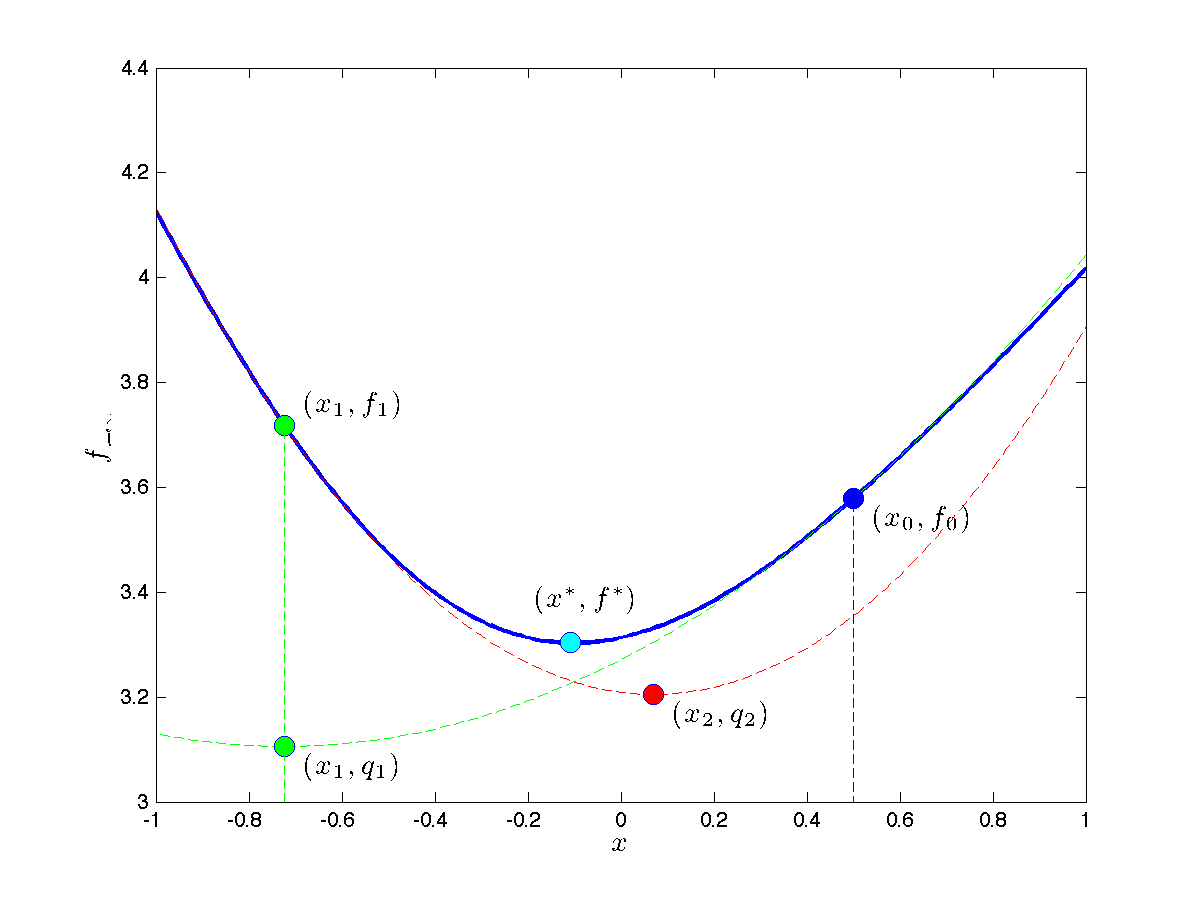
\includegraphics[width=0.66\textwidth]{img/cp_newton_conv.png}
\end{center}

\end{frame}

%%%%%%%%%%%%%%%%%%%%%%%%%%%%%%%%%%%%%%%%%%%%%%%%%%%
\begin{frame}[fragile] \frametitle{} \oldB \small

\textbf{\yblue{Momentum}}

The problem with second order methods is that the require learning
a $p$-by-$p$ matrix of values. This can be huge for modern neural
networks. An alternative approach is to use a concept similar to
the physical idea of momentum. Specifically, we use updates of
the form
\begin{align*}
v_{t+1} &= \mu \cdot v_{t} - \eta \cdot \nabla f(\beta_{t}) \\
\beta_{t+1} &= \beta_{t} + v_{t+1}.
\end{align*}
Where the value $\mu \in [0,1]$ serves as proxy for friction.

This conveniently requires only a minimal increase in complexity
but drastically increases the performance of fitting neural networks.

\end{frame}


%%%%%%%%%%%%%%%%%%%%%%%%%%%%%%%%%%%%%%%%%%%%%%%%%%%
\begin{frame}[fragile] \frametitle{} \oldB \small

\textbf{\yblue{Nesterov's Method}}

A slight tweak of standard momentum, which is also important
when optimizing non-convex surfaces, is to use Nesterov's Method.
This calculates the gradient at the spot that would be arrived
at with the current momentum. Specifically:
\begin{align*}
v_{t+1} &= \mu \cdot v_{t} - \eta \cdot \nabla f(\beta_t + \mu \cdot v_{t}) \\
\beta_{t+1} &= \beta_{t} + v_{t+1}.
\end{align*}
A picture helps considerably in understanding this.

\end{frame}

%%%%%%%%%%%%%%%%%%%%%%%%%%%%%%%%%%%%%%%%%%%%%%%%%%%
\begin{frame}[fragile] \frametitle{} \oldB \small

\textbf{Nesterov's Method}

\begin{center}
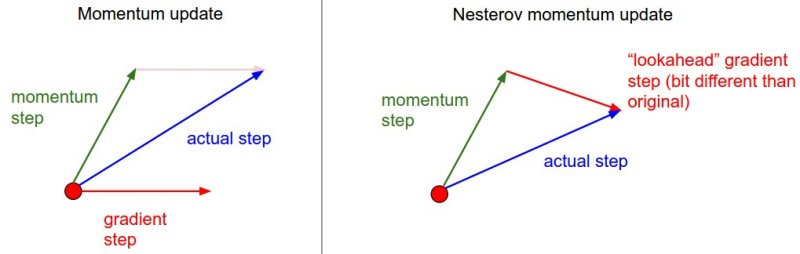
\includegraphics[width=\textwidth]{img/nesterov.jpeg}
\end{center}

\end{frame}

%%%%%%%%%%%%%%%%%%%%%%%%%%%%%%%%%%%%%%%%%%%%%%%%%%%
\begin{frame}[fragile] \frametitle{} \oldB \small

\textbf{\yblue{Learning Rate Annealing}}

As we have already seen, it is necessary to decrease the learning
rate $\eta$ over time in stochastic gradient descent. In the SVM
case we have used a $1/t$ decay, where $t$ is the epoch number.
Other popular suggestions are to use $e^{-kt}$ or to use $(1 - ts)$
for some step size $s$.

Karpathy suggests that the fixed step size is the most popular at
the moment, when only using a single learning rate.

\end{frame}

%%%%%%%%%%%%%%%%%%%%%%%%%%%%%%%%%%%%%%%%%%%%%%%%%%%
\begin{frame}[fragile] \frametitle{} \oldB \small

\textbf{\yblue{Adaptive learning rates}}

Another approach is to adaptively decay the learning rate for each
parameter by tracking how fast the gradient is changing. A popular
example is \textbf{Adagrad}, seen here:
\begin{quote}
Duchi, J., Hazan, E., \& Singer, Y. (2011). Adaptive subgradient methods for online learning and stochastic optimization. The Journal of Machine Learning Research, 12, 2121-2159.
Chicago
\end{quote}
Or \textbf{Adam}, given in this paper:
\begin{quote}
Kingma, D., \& Ba, J. (2014). Adam: A method for stochastic optimization. arXiv preprint arXiv:1412.6980.
\end{quote}
Both are quite readable and I suggest taking a look if you would like
more details. Currently, many other heuristics are also used and this
is an active area of interest (with a lack of theoretical understanding).

\end{frame}

%%%%%%%%%%%%%%%%%%%%%%%%%%%%%%%%%%%%%%%%%%%%%%%%%%%
\begin{frame}[fragile] \frametitle{} \oldB \small

\textbf{\yblue{A look ahead}}

We now actually have a clean picture of the basic structure of a neural
network. After the past two classes, we have also seen many of the standard
tricks for learning the high-dimensional, non-convex optimization function
required for fitting the weights and biases in a neural network.

After the break, we will cover:
\begin{itemize}
\item the keras library, a python module for building and fitting neural networks
much more efficiently
\item convolutional modules (or CNNs)
\item recurent modules (or RNNs)
\end{itemize}
Note that the last two things are simply different module types, other than
the linear, activation, or cost layers. Historically they are described as
different \textit{types} of neural networks, but I do not feel that is a
fruitful way of thinking about them.

\end{frame}


\end{document}











